\chapter[Scarefault]{Scarefault}
Neste capítulo será abordado o \Scarefault, o produto final desse
trabalho. Este capítulo está dividido em seções. A primeira seção aborda
uma visão geral do \Scarefault. A segunda seção faz uma análise da
arquitetura do \framework e suas dependências. Na seção seguinte explana-se
a respeito da utilização do \Scarefault.

\section{\Scarefault: Visão Geral}
O \scarefault é um \framework que tem a intenção de gerar testes unitários
de forma semiautomatizada. Para isso, ele necessita da intervenção do
desenvolvedor que o utiliza por meio de breves especificações nos
comentários de documentação. A partir dessas especificações o \scarefault
coleta informações necessárias para a produção dos casos de teste e gera
um arquivo contendo os testes solicitados. É importante ressaltar que,
para esse trabalho, os testes gerados são apenas testes caixa preta.

O \framework se propõe em permitir a acoplagem de diferentes linguagens
de programação. Para isso, há a necessidade da construção de um \parser
que identifique a sintaxe da linguagem alvo por meio de duas
ferramentas: \flexcpp e \textsf{Bisonc++}. Essas duas ferramentas são
comuns em contextos de produção de compiladores. Com o \parser
implementando o desenvolvedor poderá implemetnar as especificidades
relacionadas aos testes da linguagem alvo, tendo como base o código
oferecido pelo \Scarefault.

O \scarefault foi escrito em \cpp e está licenciado dentro das condições
da \textsf{GPLv3}. Todo o seu código fonte encontra-se em:
\url{https://github.com/Scarefault/scarefault}.

\section{A Arquitetura do \scarefault}
Essa seção evidencia os elementos da arquitetura do \Scarefault. Como
ele foi desenhado, quais conceitos foram utilizados e como ele funciona.
Em um primeiro momento são exploradas visões estáticas da arquitetura,
para então mostrar o \scarefault dinamicamente.

\subsection{Visão de Pacotes}
Partindo-se de uma visão macroscópica, o \scarefault pode ser dividido em
dois módulos básicos: o \textsf{identificador} e o \textsf{gerador}. A Figura
\ref{modules-scarefault} ilustra esses módulos básicos.

\begin{figure}[h]
  \centering
    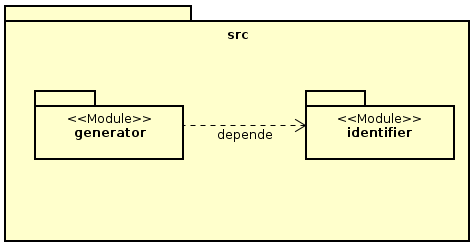
\includegraphics[width=0.6\textwidth]{figuras/modules-scarefault.png}
    \caption{Representação dos módulos do \Scarefault}
    \label{modules-scarefault}
\end{figure}
\FloatBarrier

\begin{description}
\item[Identificador:] é responsável pela identificação das regras que regem
a gramática da linguagem de programação alvo, bem como da coleta dos dados
necessários para a produção dos casos de teste.
\item[Gerador:] responsável pela geração dos casos de teste. A partir dos dados
coletados das especificações do desenvolvedor e do próprio código fonte, esse
módulo é capaz de gerar casos de teste.
\end{description}

Expandindo-se os módulos pode-se observar os pacotes associados a cada um deles
e o relacionamento entre esses pacotes, como mostra a Figura
\ref{expand-modules-scarefault-1}.

\begin{figure}[h]
  \centering
    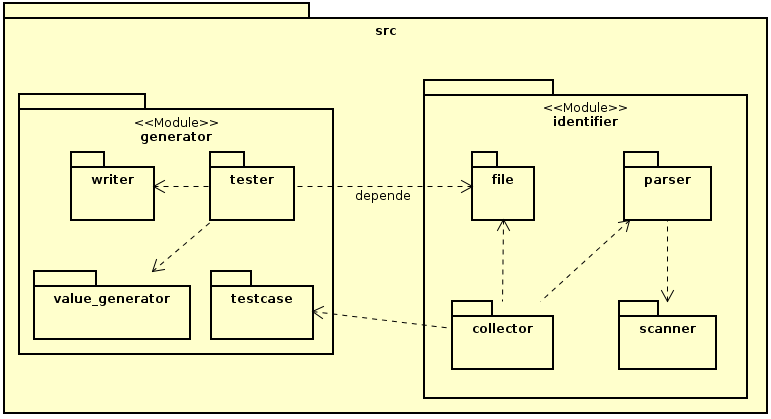
\includegraphics[width=0.8\textwidth]{figuras/expand-modules-scarefault-1.png}
    \caption{Representação expandida dos módulos do \Scarefault}
    \label{expand-modules-scarefault-1}
\end{figure}

Como indicado na Figura \ref{expand-modules-scarefault-1}, os pacotes associados ao
módulo \textsf{identifier} são:
\begin{description}
\item[\textit{scanner}:] responsável pela análise léxica do arquivo contendo o código
fonte em avaliação. As classes contidas nesse pacote são geradas pelo \flexcpp durante
a compilação.
\item[\textit{parser}:] responsável pela análise sintática do arquivo contendo o
código em avaliação. As ações que ele executa quando determinada regra gramatical é
encontrada são, essencialmente, ações de coleta de dados. As classes associadas
a esse pacote são geradas pelo \bisoncpp durante a compilação.
\item[\textit{collector}:] responsável pela coleta de dados necessários para a
criação de testes unitários.
\item[\textit{file}:] responsável por guardar os dado coletados do código fonte.
Dados como as dependências (\textit{libraries} importadas), métodos e classe
do arquivo em análise.
\end{description}

Os pacotes associados ao módulo \textsf{generator}, como mostra a Figura
\ref{expand-modules-scarefault-1}, são:
\begin{description}
\item[	\textit{tester}:] responsável pela construção dos arquivos de teste. A partir
dele é que os testes ganham forma, conforme a linguagem de programação.
\item[	\textit{testecase}:] responsável por guardar os dados relacionados
a cada caso de teste especificado pelo desenvolvedor, a partir dos
comentários no código fonte.
\item[	\textit{value\_generator}:] responsável por gerar valores randômicos
para o desenvolvimento dos testes.
\item[\textit{writer}:] responsável por escrever as informações da arquivo de
teste, enviadas pelo \textsf{tester}. Para isso, ele cria o arquivo e
escreve todas as informações a ele solicitadas.
\end{description}

\subsection{Visão de Classes}
As Figuras \ref{modules-scarefault} e \ref{expand-modules-scarefault-1} mostram
a visão de pacotes do \scarefault e como eles se relacionam, bem como a
responsabilidade que cabe a cada um deles. Aprofundando-se mais, chega-se a uma
visão das entidades associadas a cada pacote. A visão de quais são essas
entidades e como elas se relacionam pode ser verificada pelo diagrama de 
domínio, mostrado na Figura \ref{domain-diagram}.
\begin{figure}[h]
  \centering
    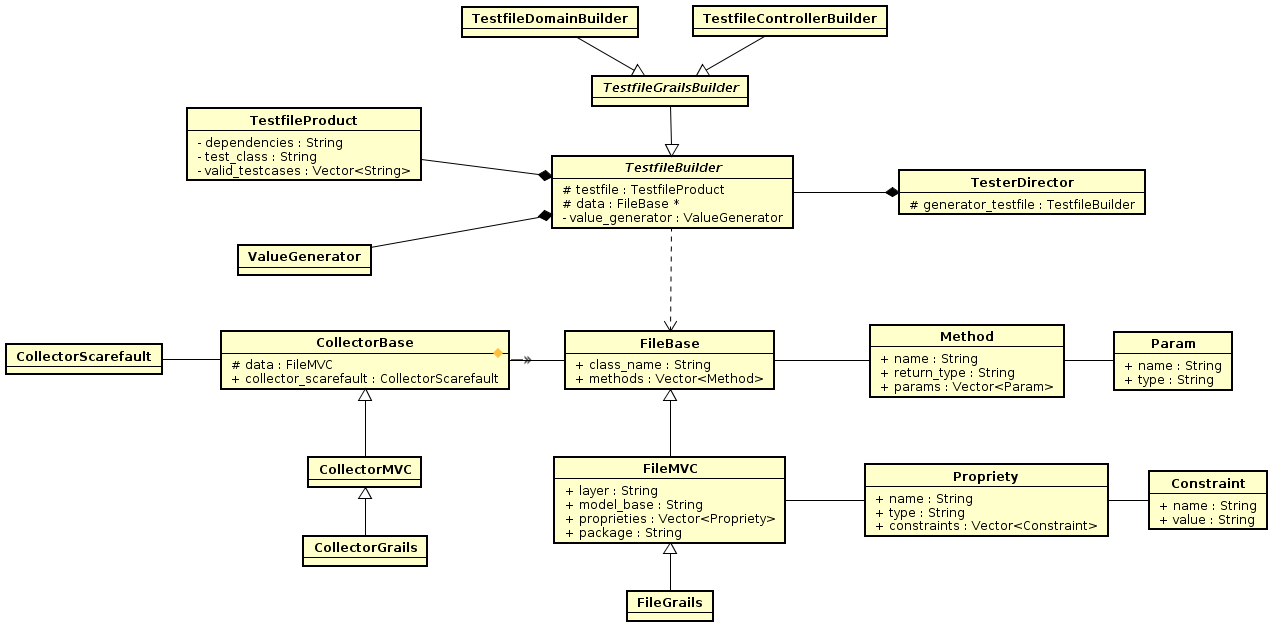
\includegraphics[width=\textwidth]{figuras/domain-diagram.png}
    \caption{Diagrama de domínio do \Scarefault}
    \label{domain-diagram}
\end{figure}
\FloatBarrier

O diagrama de domínio na Figura \ref{domain-diagram} demonstra a relação
entre as principais entidades que o \framework trabalha. O \textsf{Collector}
recolhe as  informações essencias para os testes a partir do
\textsf{Parser} que, por sua vez, recebe um \textit{stream} de dados a partir
do \textsf{Scanner}. Como dados importantes para a produção de testes pelo
\scarefault tem-se métodos (\textsf{Method}) e seus parâmetros (\textsf{Param})
e, para arquiteturas voltadas ao MVC, tem-se propriedades (\textsf{Propriety})
e suas restrições (\textsf{Constraint}). Esses dados estão intimamente ligados
ao arquivo em análise, portanto, são armazenados na entidade arquivo (\textsf{FileBase}).
Há também a entidade \textsf{TestCase} que tem papel fundamental na produção
dos testes, pois carrega as informações dispostas pelo desenvolvedor sobre os
testes a serem criados. Uma parte importante dos casos de teste são os
argumentos (\textsf{Arg}) que devem ser passados ao método em teste durante o
teste.

Partindo-se do diagrama de domínio exposto na Figura \ref{domain-diagram}, pode-se
visualizar o diagrama de classe, mostrado na Figura \ref{class-diagram}.
%\begin{landscape}
\begin{figure}[h]
  \centering
    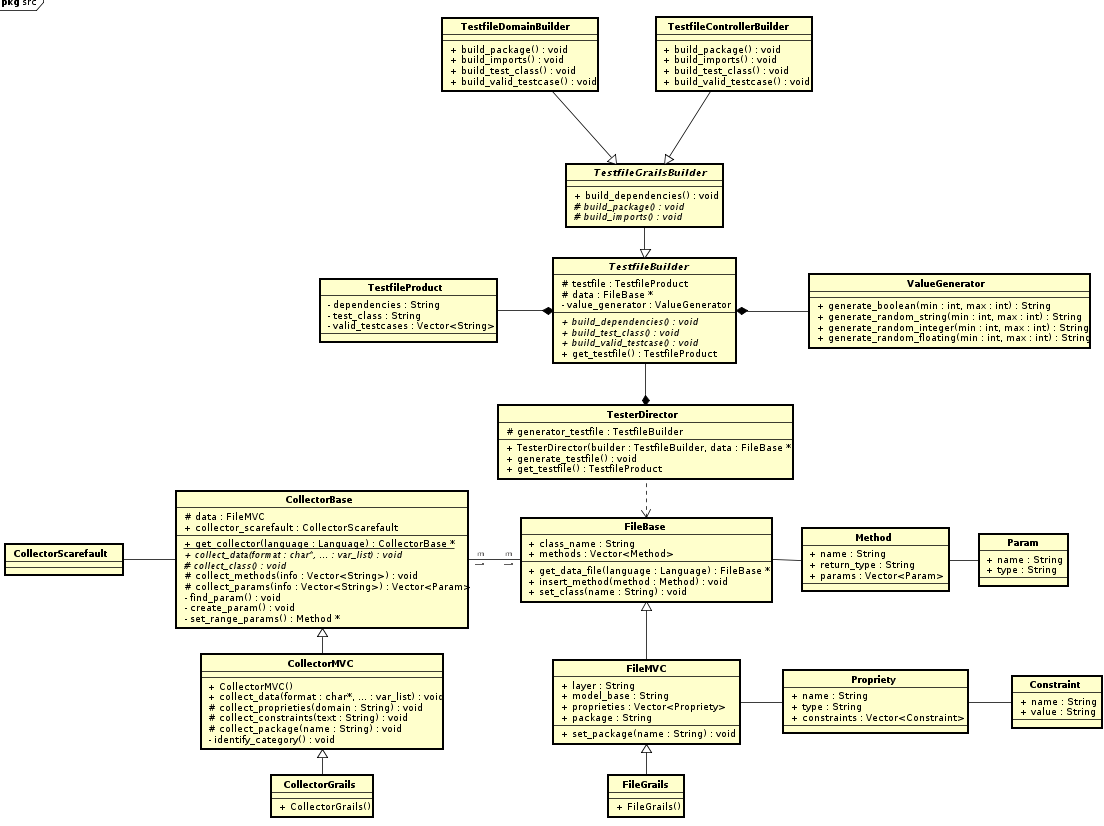
\includegraphics[width=\textwidth]{figuras/class-diagram.png}
    \caption{Diagrama de classe completo do \Scarefault}
    \label{class-diagram}
\end{figure}
\FloatBarrier
%\end{landscape}

O diagrama de classes permite obter uma visualização mais apurada dos
relacionamentos entre as classes contidas no \textit{framework}. As principais
entidades do \textit{framework}, apresentadas na Figura \ref{domain-diagram},
estão presentes e muitas delas passaram a ter um conjunto de classes auxiliar,
de forma a permitir a sua adaptação ao contexto em que será inserida.

Por meio da Figura \ref{class-diagram} pode-se identificar o uso de alguns
\textit{design patterns} de criação e de estrutura, com o intuito de 
permitir a extensibilidade do \framework e a sua facilidade de uso.
Para esse fim, foram usados os conceitos do \textbf{\textit{builder pattern}} e
\textbf{\textit{factory pattern}}.

\section{A Utilização do \scarefault}